\subsection{Raspberry Pi}
Several generations of Raspberry Pis have been released. The first generation (Raspberry Pi 1 Model B) was released in February 2012. It was followed by a simpler and inexpensive model Model A. In 2014 the foundation released a board with an improved design in Raspberry Pi 1 Model B+. The model laid the current "mainline" form-factor. Improved A+ and B+ models were released a year later. A cut down "compute" model was released in April 2014, and a Raspberry Pi Zero with smaller size and limited input/output (I/O) and general-purpose input/output (GPIO) abilities was released in November 2015 for US\$5. The Raspberry Pi 2 which added more RAM was released in February 2015. Raspberry Pi 3 Model B released in February 2016 is bundled with on-board WiFi and Bluetooth. As of 2016, Raspberry Pi 3 Model B is the newest mainline Raspberry Pi. These boards are priced between US \$20–35.\\
All models feature a Broadcom system on a chip (SoC), which includes an ARM compatible central processing unit (CPU) and an on chip graphics processing unit (GPU, a VideoCore IV). CPU speed ranges from 700 MHz to 1.2 GHz for the Pi 3 and on board memory range from 256 MB to 1 GB RAM. Secure Digital (SD) cards are used to store the operating system and program memory in either the SDHC or MicroSDHC sizes. Most boards have between one and four USB slots, HDMI and composite video output, and a 3.5 mm phone jack for audio. Lower level output is provided by a number of GPIO pins which support common protocols like I²C. The B-models have an 8P8C Ethernet port and the Pi 3 has on board Wi-Fi 802.11n and Bluetooth.\\
The Foundation provides Raspbian, a Debian-based Linux distribution for download, as well as third party Ubuntu, Windows 10 IOT Core, RISC OS, and specialised media center distributions. It promotes Python and Scratch as the main programming language, with support for many other languages. The default firmware is closed source, while an unofficial open source is available.
The Raspberry Pi 3 model was used for preliminary development of this driver.
\begin{figure}[H]
	\centering
	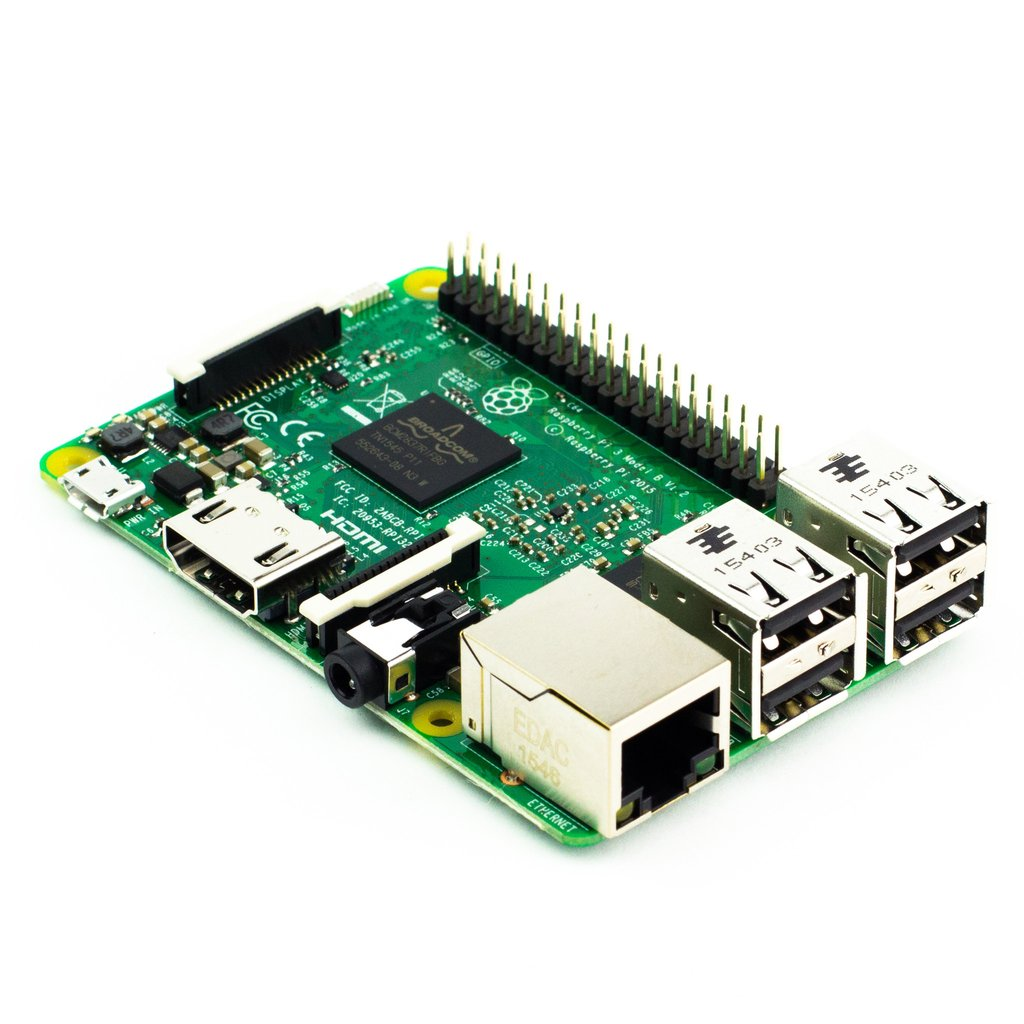
\includegraphics[width=3.5in, height=3in]{images/raspberry_pi.png}
	\caption{Raspberry Pi 3}
\end{figure}
